\documentclass{article}
\usepackage{indentfirst}
\usepackage[utf8]{inputenc}
\usepackage[T1]{fontenc}
\usepackage{lmodern}
\usepackage{graphicx}
\usepackage{float}
\usepackage[]{subfigure}
\usepackage{afterpage}
\usepackage{amsmath}
\usepackage{gensymb}

\usepackage[brazilian]{babel}


\usepackage{listings}
\usepackage{color}

\definecolor{dkgreen}{rgb}{0,0.6,0}
\definecolor{gray}{rgb}{0.5,0.5,0.5}
\definecolor{mauve}{rgb}{0.58,0,0.82}

\lstset{frame=tb,
  language=Matlab,
  aboveskip=3mm,
  belowskip=3mm,
  showstringspaces=false,
  basicstyle={\small\ttfamily},
  numbers=none,
  numberstyle=\tiny\color{gray},
  keywordstyle=\color{blue},
  commentstyle=\color{dkgreen},
  stringstyle=\color{mauve},
  breaklines=true,
  breakatwhitespace=true,
  tabsize=4
}


\addtolength{\topmargin}{-.750in}
\addtolength{\textheight}{1.5in}


\title{Simulação 4 - Controle Digital}
\author{Arthur de Matos Beggs - 12/0111098}
\date{}

\begin{document}

%\maketitle

% capa
\begin{titlepage}
    \begin{center}
        \centering
        
\includegraphics[width=1\linewidth]{images/LogoUnB.png}\\[1cm]
        {\large \textbf{Universidade De Brasília}}\\[0.2cm]
        {\large \textbf{Departamento De Engenharia Elétrica}}\\[0.2cm]
        {\large \textbf{Controle Digital}}\\[5.1cm]
        {\bf \huge Simulação 4}\\[5.1cm]
    \end{center}
{\large Aluno: \\    Arthur de Matos Beggs ----------------------------------------- 12/0111098 }
\vspace{7mm}
    \begin{center}
        {\large 1º/2020}
    \end{center}
\end{titlepage}

\clearpage % Quebra de página

\setcounter{page}{2}

    \begin{figure}[H]
       \centering
            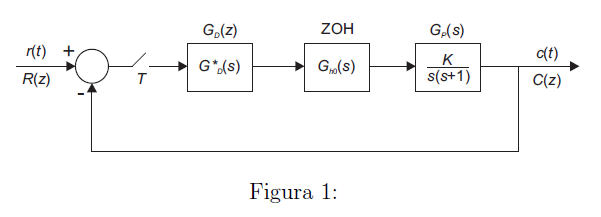
\includegraphics[width=1\linewidth]{images/Diagrama.png}
            \caption{Diagrama e funções de transferência do sistema.}
            \label{fig:diagram}
    \end{figure}

\section*{Questão 1}

    $$ G(z) = \mathcal{Z}\left\{\frac{ 1 - \mathrm{e}^{-0.2s} }{s} \frac{K}{s(s+1)} \right\} = (1-z^-1) \mathcal{Z}\left\{ \frac{K}{s^{2} (s+1)}  \right\} = 0.01873\left[ \frac{ K(z+0.9356) }{ (z-1)(z-0.8187) } \right] $$\\[0.1cm]

    $$ G(z) = \frac{ K(0.01873z + 0.01752) }{ z^{2}-1.8187z+0.8187 } $$\\[0.1cm]

    {Para $ G(\omega) = G(z) |_{z = \frac{ 1+0.1\omega }{ 1-0.1\omega }} $ :}\\[0.1cm]

    $$ G(\omega) = \frac{ K\left[0.01873\left(\frac{ 1+0.1\omega }{ 1-0.1\omega }\right) + 0.01752\right] }{ \left(\frac{ 1+0.1\omega }{ 1-0.1\omega }\right)^{2}-1.8187\left(\frac{ 1+0.1\omega }{ 1-0.1\omega }\right)+0.8187 } = \frac{ K(-0.000333\omega^{2} -0.09633\omega +0.9966) }{ \omega^{2} +0.9969\omega } $$\\[0.1cm]

    $$ G(\omega) \doteq \frac{ K\left( 1+\frac{\omega}{300} \right)\left( 1-\frac{\omega}{10} \right) }{ \omega( \omega +1 ) } $$\\[0.2cm]

\section*{Questão 2}
    {Para o compensador em avanço $ G_{D}(\omega) = \frac{ 1 + \tau\omega }{ 1 + \alpha\tau\omega }, 0<\alpha<1 $ :}\\[0.1cm]

    $$ K_{v} = \lim_{\omega \to 0} \omega G_{D}(\omega)G(\omega) \doteq K = 2 $$\\[0.2cm]

\section*{Questão 3}
    \begin{figure}[H]
       \centering
            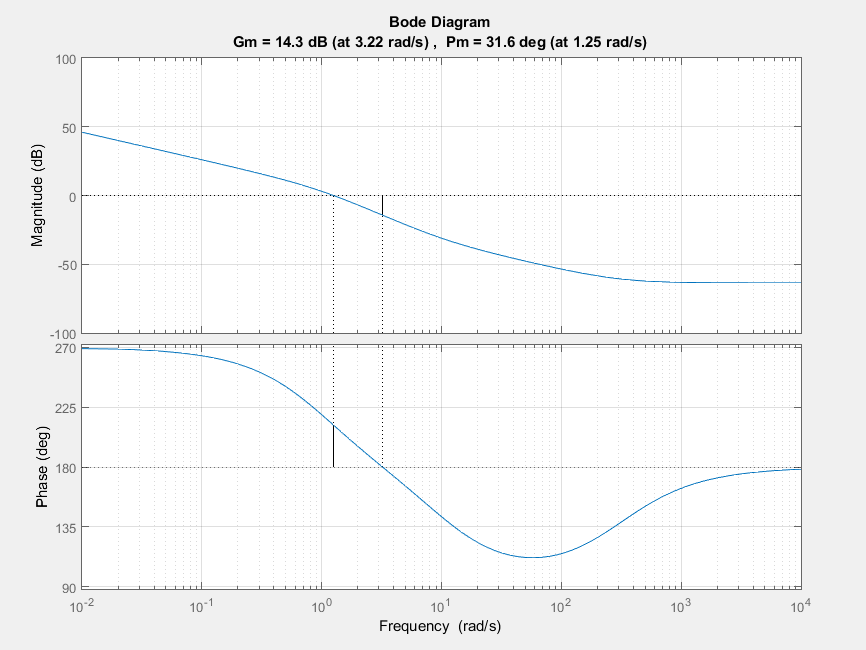
\includegraphics[width=1\linewidth]{images/bodeG.png}
            \caption{Diagrama de Bode de $ G(s) = G(\omega)|_{\omega=s} $}
            \label{fig:bodeG}
    \end{figure}

\section*{Questão 4}
    {A Margem de Fase de $G (\omega) $ é de $ 31.6 ^{\circ} $. Para que a Margem de Fase satisfaça o requerimento de $ 50 ^{\circ} $, um avanço de fase de $ \approx 20 ^{\circ} $ é necessário. Porém, também é necessário compensar o deslocamento da frequência de cruzamento. Assim, $ 8 ^{\circ} $ adicionais compensam a frequência de cruzamento, resultando em $ \phi_m = 28 ^{\circ} $. Com isso,}

    $$ \phi_m = \frac{ 1-\alpha }{ 1+\alpha } \implies \alpha = 0.361. $$

    $$ -20 log\frac{ 1 }{ \sqrt{\alpha} } = -20 log \frac{ 1 }{ \sqrt{ 0.361 } } = -4.425 dB $$\\[0.05cm]

    {Por tentativa e erro, temos}

    $$ v_{m} = \frac{1}{ \sqrt{\alpha}\tau } \approx 1.7 $$\\[0.05cm]

    {Assim, $ \tau \approx 0,979 $ e}

    $$ G_{D}(\omega) = \frac{ 1+\tau\omega }{ 1+\alpha\tau\omega } = \frac{ 1 + 0.9790\omega }{ 1 + 0.3534\omega } $$\\[0.2cm]

    {Transformando para o plano \textit{z},}

    $$ \omega = \frac{2}{0.2} \frac{z-1}{z+1} = 10\frac{z-1}{z+1} $$

    $$ G_{D}(z) = \frac{ 1 + 0.9790 \left( 10\frac{z-1}{z+1} \right) }{ 1 + 0.3534 \left( 10\frac{z-1}{z+1} \right) } = \frac{ 2.3798z - 1.9387 }{ z - 0.5589 } $$

    $$ G_{D}(z)G(z) = \frac{ 2.3798z - 1.9387 }{ z - 0.5589 } \frac{ 2(0.01873z + 0.01752) }{ z^{2}-1.8187z+0.8187 } $$

    $$ G_{D}(z)G(z) = \frac{ 0.0891z^2 +0.0108z -0.0679 }{ z^3 -2.3776z^2 +1.8352z -0.4576 } $$

\section*{Questão 5}
    \begin{figure}[H]
       \centering
            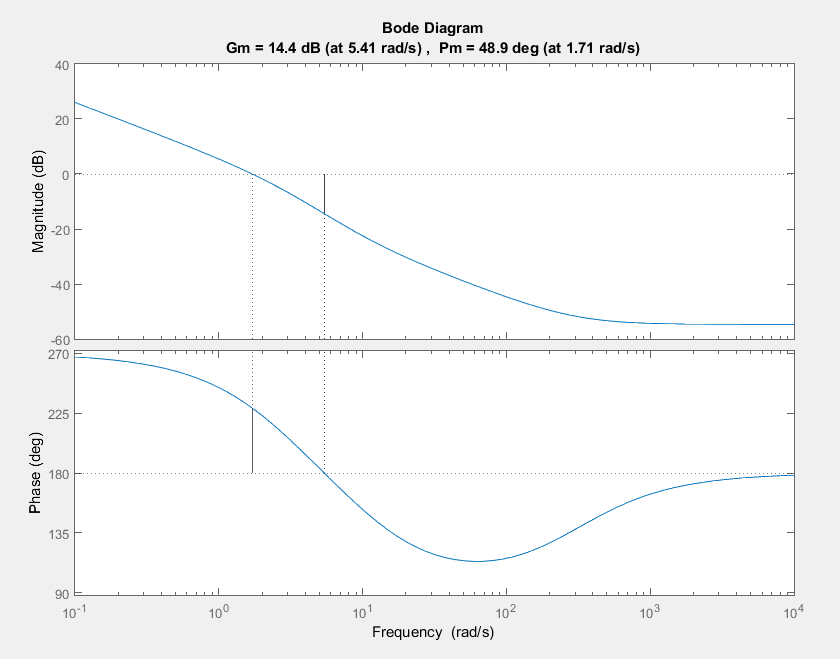
\includegraphics[width=1\linewidth]{images/bodeGdG.png}
            \caption{Diagrama de Bode de $ G_{D}(s)G(s) = G_{D}(\omega)G(\omega)|_{\omega=s} $}
            \label{fig:bodeGdG}
    \end{figure}

    {O diagrama de Bode de $ G_{D}(s)G(s) = G_{D}(\omega)G(\omega)|_{\omega=s} $ apresenta Margem de Ganho de 14.4 dB (>10 dB, conforme requisito de projeto) e Margem de Fase de $ 48.9 ^{\circ} $($     \approx 50 ^{\circ} $, conforme requisito de projeto). Assim, o controlador em avanço projetado apresenta Margens de Ganho e Fase muito próximas ao esperado, satisfazendo as especificações.}



\end{document}
